\section{Shifting Process in Response to COVID-19}

Following the COVID-19 closure, the SSDT was ended for the remainder of the Spring 2020 term. Only the leadership team continued to work on the software systems in our last sprint. The shutdown itself required a few changes to existing systems. For example, updated syllabi were needed for every course, outlining how classes would change during emergency online teaching. One of our software systems was currently being used to collect syllabi during regular terms; our team quickly modified the system to support an addition, ``odd'' term, where faculty could quickly and easily upload new syllabi.

The SSDT team worked with the administration to permit students to work on software in a remote-only capacity. The team quickly adapted its framework to this new work environment. One of the many considerations that had to be acknowledged during this process is that some students were now dealing with outside distractions that did not exist when working in our space, including moving back in with their families, balancing parenting and other duties, and unreliable technology at home.

The leadership team prepared by reprioritizing all of the remaining issues in the queue. They then did a thorough walkthrough of the current application to identify new issues, as some work was unfinished as students left campus in a hurry. The final and most important step was deciding which tools the team would use that would most closely resemble the workflow that existed while on-campus. Ultimately, the leadership team identified four tools that were key to facilitating student success in a remote SSDT environment: 1) a digital version of the Kanban board for organizing tasks; 2) a communication platform to facilitate online meetings; 3) a wireframing tool for creating low fidelity prototypes, replacing our paper prototyping process; and 4) a collaborative code editor for modeling pair programming. The next section details how these tools were implemented.

\subsection{New Tools and Processes}
Above all else, constant and consistent communication between the students and the leadership team was of the utmost importance. Having good visibility on what everyone was working on would be the first step in ensuring progress. An online Kanban board was used to digitize the physical board in our space. Figure~\ref{fig:digitalkanban} shows the old and new versions of the Kanban board, indicating related objects on each.

\begin{figure}[h]
 \centering
 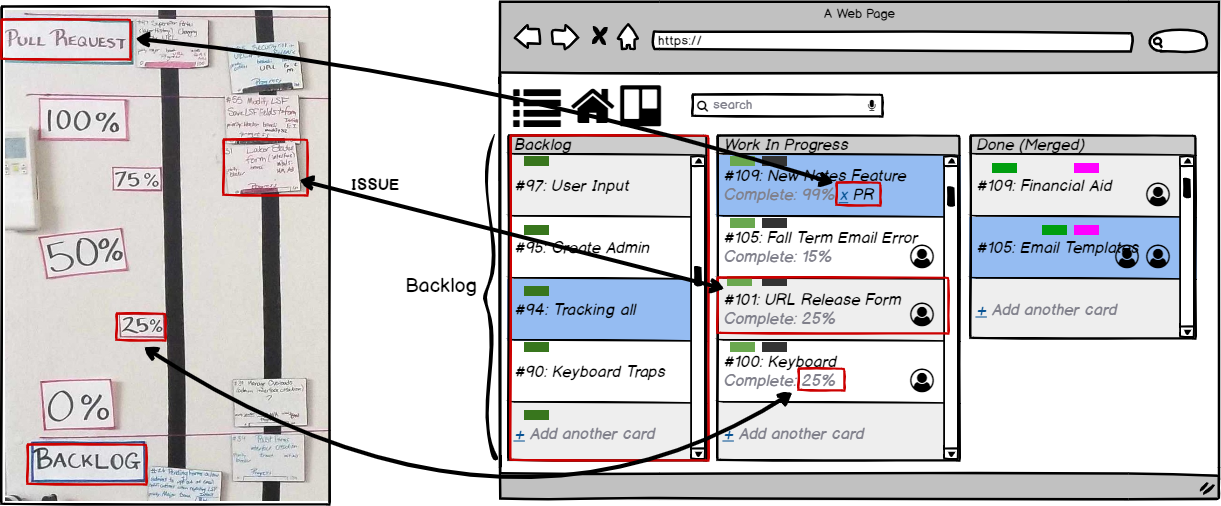
\includegraphics[width=0.8\linewidth]{newTrellomockup2.png}
 \caption{The physical Kanban board (left) and its virtual equivalent (right)}
 \label{fig:digitalkanban}
\end{figure}

The team already utilized a communication platform for much of its online communication, so it was decided to continue with a more significant reliance on this tool. The student programmers followed a ``Did, Doing, Stuck'' (DDS) structure, where the students would explain what they did the previous day, what they will be doing this work day, and if they are stuck on anything. The leadership team would check these updates daily to monitor progress and ensure students are not stuck for an extended amount of time, closely mirroring our process before the crisis. The communication platform also offered video calling capabilities, allowing the team to continue doing Scrum meetings as they did in the previous summers, just through video conferencing. Screensharing was leveraged to simulate whiteboards, and share interfaces for feedback.

Given the situation, students were not able to collaborate in-person on paper prototypes. Instead, an online collaborative wireframing tool was used to create mockups. The wireframing tool proved nearly as effective as paper prototyping, because it allowed designs to be responsive and perform like actual webpages (e.g., demonstrating ``on click" events). This ensured that the team did not stray from our design standards, and introduced a tool that provides an efficient way to prototype interfaces that will be adopted post-pandemic.

Students used to work in pairs at a single workstation, alternating between driver and navigator. Pair programming was particularly important to the leadership team, as it teaches the students the importance of working with others and asking questions. Our solution was for the student programmers to video call during the entire work session, allowing them to discuss their work, similar to before the crisis. However, pair programming from different terminals is highly ineffective. So, a plugin was added to their IDEs that allowed pairs to share code and see edits in real-time. The leadership team also used this plugin to perform code reviews with the student teams.

Anecdotal evidence suggests that the students are feeling productive, efficient, and are still learning a lot from the experience. The leadership team regularly asks the students in the morning scrum meetings to provide feedback about how to improve this process for them. They are mostly indicating they simply need practice and time to develop the skills needed, which is largely in line with what is expected of them when in person.
